% Especificação Detalhada — versão 3 (2026-09-27)
% Reconstruída a partir do PDF da v2, com as alterações de
% docs/especificacao_v3_alteracoes.md (decisões D-001 a D-004 do CLAUDE.md).
%
% Compilar (na pasta docs/especificacao):
%   pdflatex especificacao && bibtex especificacao && pdflatex especificacao && pdflatex especificacao
% ou simplesmente: latexmk -pdf especificacao

\documentclass[12pt, oneside, a4paper, english, brazil]{abntex2}

\usepackage[utf8]{inputenc}
\usepackage[T1]{fontenc}
\usepackage{lmodern}
\usepackage{amsmath, amssymb}
\usepackage{booktabs}
\usepackage{array}
\usepackage{tabularx}
\usepackage{float}
\usepackage{tikz}
\usetikzlibrary{arrows.meta}
\usepackage[alf]{abntex2cite}
\hypersetup{hidelinks} % hyperref já é carregado pela classe abntex2

% ---------------------------------------------------------------------------
% Dados do trabalho
% ---------------------------------------------------------------------------
\titulo{Aplicação de Protocolos de Oblivious Transfer para Preservação de Privacidade em Transações Digitais}
\autor{João Paulo Garcia, João Pedro Magalhães, Miguel Luis Schwengber}
\local{São Paulo, SP}
\data{2026}
\orientador{Prof. Dr. Thales Areco Bandiera Paiva}
\preambulo{Trabalho de conclusão de curso apresentado ao Departamento de
Engenharia de Computação e Sistemas Digitais da Escola Politécnica da
Universidade de São Paulo para obtenção do Título de Engenheiro.}

% ---------------------------------------------------------------------------
% Diagramas de sequência (TikZ)
% ---------------------------------------------------------------------------
% Posição horizontal das linhas de vida (cm)
\def\xCli{0}
\def\xAdm{2.1}
\def\xWeb{4.8}
\def\xGat{7.4}
\def\xCdn{9.8}
\def\xPrg{12.4}

\tikzset{
  sdmsg/.style={-{Stealth[length=2mm]}, thin},
  sdret/.style={sdmsg, dashed},
  sdlbl/.style={font=\scriptsize, inner sep=1pt, fill=white},
}

% cabeçalhos
\newcommand{\sdactor}[2]{%
  \draw (#1,0.75) circle (0.13);
  \draw (#1,0.62) -- (#1,0.3);
  \draw (#1-0.18,0.5) -- (#1+0.18,0.5);
  \draw (#1-0.15,0.05) -- (#1,0.3) -- (#1+0.15,0.05);
  \node[font=\small] at (#1,-0.2) {#2};}
\newcommand{\sdhead}[2]{%
  \node[draw, font=\small, align=center, fill=white] at (#1,-0.1) {#2};}
\newcommand{\sdlifelines}[1]{%
  \foreach \x in {\xCli,\xAdm,\xWeb,\xGat,\xCdn,\xPrg}
    \draw[dashed, gray] (\x,-0.5) -- (\x,#1);}
\newcommand{\sdheads}{%
  \sdactor{\xCli}{Cliente}
  \sdactor{\xAdm}{Administrador}
  \sdhead{\xWeb}{Sistema Web}
  \sdhead{\xGat}{Gateway de\\Pagamento}
  \sdhead{\xCdn}{CDN}
  \sdhead{\xPrg}{Programa Local}}

% mensagens: {origem}{destino}{y}{rótulo}
\newcommand{\sdcall}[4]{\draw[sdmsg] (#1,#3) -- (#2,#3) node[sdlbl, midway, above] {#4};}
\newcommand{\sdreply}[4]{\draw[sdret] (#1,#3) -- (#2,#3) node[sdlbl, midway, above] {#4};}
% automensagem: {linha}{y}{rótulo}; R = rótulo à direita, L = à esquerda
\newcommand{\sdselfR}[3]{%
  \draw[sdmsg] (#1,#2) -- ++(0.35,0) -- ++(0,-0.3) -- ++(-0.35,0);
  \node[sdlbl, anchor=west, align=left] at (#1+0.45,#2-0.15) {#3};}
\newcommand{\sdselfL}[3]{%
  \draw[sdmsg] (#1,#2) -- ++(0.35,0) -- ++(0,-0.3) -- ++(-0.35,0);
  \node[sdlbl, anchor=east, align=right] at (#1-0.1,#2-0.15) {#3};}

% faixa de seção: {y}{título}
\newcommand{\sdbanner}[2]{%
  \draw[double, thick] (-1,#1) -- (13.6,#1);
  \node[draw, fill=white, font=\small\bfseries] at (6.3,#1) {#2};}
% bloco combinado: {x1}{y topo}{x2}{y base}{tipo}{guarda}
\newcommand{\sdframe}[6]{%
  \draw (#1,#2) rectangle (#3,#4);
  \node[draw, anchor=north west, font=\scriptsize\bfseries, inner sep=2pt, fill=white] (sdk) at (#1,#2) {#5};
  \node[anchor=west, font=\scriptsize\bfseries] at (sdk.east) {[#6]};}
% separador de alternativa: {x1}{x2}{y}{guarda}
\newcommand{\sdelse}[4]{%
  \draw[dashed] (#1,#3) -- (#2,#3);
  \node[anchor=north west, font=\scriptsize\bfseries] at (#1,#3) {[#4]};}

% ---------------------------------------------------------------------------
\begin{document}

\selectlanguage{brazil}
\frenchspacing

% ---------------------------------------------------------------------------
% Capa e folha de rosto
% ---------------------------------------------------------------------------
\begin{capa}
  \begin{center}
    {\large \imprimirautor}
    \vspace*{\fill}

    {\ABNTEXchapterfont\bfseries\LARGE \imprimirtitulo}
    \vspace*{\fill}

    {\large \imprimirlocal}\par
    {\large \imprimirdata}
    \vspace*{1cm}
  \end{center}
\end{capa}

\begin{center}
  \thispagestyle{empty}
  {\large \imprimirautor}
  \vspace*{\fill}

  {\ABNTEXchapterfont\bfseries\Large \imprimirtitulo}
  \vspace*{\fill}

  \hspace{.45\textwidth}
  \begin{minipage}{.5\textwidth}
    \SingleSpacing\small \imprimirpreambulo
  \end{minipage}
  \vspace*{\fill}

  Universidade de São Paulo -- USP\par
  Escola Politécnica\par
  Departamento de Engenharia de Computação e Sistemas Digitais (PCS)
  \vspace*{\fill}

  Orientador: \imprimirorientador
  \vspace*{\fill}

  \imprimirlocal\par
  \imprimirdata
\end{center}
\cleardoublepage

% ---------------------------------------------------------------------------
\pdfbookmark[0]{\contentsname}{toc}
\tableofcontents*
\cleardoublepage

\textual

% ===========================================================================
\chapter{Introdução}
% ===========================================================================

Este documento apresenta o projeto de formatura intitulado ``Aplicação de
Protocolos de Oblivious Transfer para Preservação de Privacidade em Transações
Digitais''.

\section{Motivação}

No cenário atual do comércio eletrônico, a coleta massiva de dados se tornou
uma prática recorrente, de forma que qualquer compra torna a navegação pela
internet uma experiência infestada de anúncios de produtos relacionados.
Embora a vantagem de marketing dessa prática seja inegável, fornecer para os
consumidores a privacidade que a maioria das lojas virtuais atualmente viola é
um aspecto de grande interesse e necessidade para a sociedade.

\section{Objetivos}

\textbf{Objetivo Geral:} Desenvolver um protótipo funcional de um sistema de
venda de ativos digitais em formato de catálogo, utilizando criptografia
baseada em Oblivious Transfer (Transferência Inconsciente) para passar chaves
de criptografia simétrica usadas para descriptografar os bens digitais
adquiridos de Rede de Distribuição de Conteúdo (Content Delivery Network --
CDN), garantindo que o servidor da loja seja incapaz de identificar quais
produtos foram acessados ou adquiridos por um comprador específico.

\textbf{Objetivos Específicos:}

\begin{itemize}
\item Modelar a arquitetura do sistema para permitir a transação segura onde a
escolha do cliente é ofuscada para o servidor.
\item Implementar o algoritmo criptográfico escolhido (como 1-out-of-N) em uma
solução com 3 componentes: site online, rede de distribuição de conteúdo (CDN)
e programa local instalado no computador do cliente.
\item Desenvolver mecanismos para validar a legitimidade da transação sem
revelar o conteúdo da compra.
\item Realizar testes de segurança e desempenho para validar a impossibilidade
de rastreamento de preferências.
\end{itemize}

\section{Justificativa}

O projeto propõe uma solução técnica para um problema crescente de privacidade
digital. O sistema permitirá que o comprador adquira produtos digitais dentre
várias opções, tendo acesso a apenas uma, mas de forma que o vendedor
permaneça matematicamente incapaz de saber qual item específico foi
selecionado pelo cliente.

A metodologia envolverá a implementação de algoritmos de Oblivious Transfer
integrados a uma interface de venda, garantindo que a loja receba o pagamento,
mas não consiga registrar históricos de compras, preferências ou interesses do
usuário, assegurando assim um elevado nível de privacidade para os
consumidores.

\section{Organização do Trabalho}

Este documento está estruturado da seguinte forma: o \autoref{cap:conceitos}
apresenta os conceitos fundamentais que embasam este projeto. O
\autoref{cap:metodo} descreve a metodologia do trabalho. O
\autoref{cap:requisitos} detalha a especificação de requisitos do sistema. O
\autoref{cap:projeto} expõe o projeto e o desenvolvimento da solução. Por fim,
o Capítulo 6 reúne as considerações finais do estudo.

% ===========================================================================
\chapter{Aspectos Conceituais}\label{cap:conceitos}
% ===========================================================================

\section{Oblivious Transfer (OT)}

\subsection{Definição}

Oblivious Transfer (OT) é um protocolo criptográfico entre duas partes:

\begin{itemize}
\item \emph{Sender} $S$, que possui um conjunto de mensagens
$X = \{x_0, x_1, \ldots, x_{n-1}\}$;
\item \emph{Receiver} $R$, que escolhe um índice $i \in \{0, \ldots, n-1\}$.
\end{itemize}

O protocolo garante que:

\begin{enumerate}
\item $R$ aprende apenas $x_i$;
\item $R$ não aprende nenhuma informação sobre $x_j$ para $j \neq i$;
\item $S$ não aprende qual índice $i$ foi escolhido.
\end{enumerate}

Formalmente, o objetivo é realizar:
\[
(x_0, \ldots, x_{n-1}),\ i \longrightarrow x_i
\]
sem violar as propriedades de privacidade.

\section{Variantes de OT}

\subsection{1-out-of-2 OT}

O caso mais simples ocorre quando o \emph{sender} possui duas mensagens:
\[
(x_0, x_1)
\]
O \emph{receiver} escolhe um bit:
\[
r \in \{0, 1\}
\]
Ao final do protocolo, o \emph{receiver} obtém:
\[
x_r
\]
sem aprender $x_{1-r}$, e o \emph{sender} não descobre o valor de $r$.

\subsection{1-out-of-n OT}

Generalização do caso anterior:

\begin{itemize}
\item \emph{Sender} possui $n$ mensagens;
\item \emph{Receiver} escolhe um índice $i \in \{0, \ldots, n-1\}$;
\end{itemize}

O \emph{receiver} obtém apenas $x_i$, mantendo as mesmas garantias de
privacidade.

\subsection{k-out-of-n OT}

Nesta variante:

\begin{itemize}
\item \emph{Sender} possui $n$ mensagens;
\item \emph{Receiver} escolhe um subconjunto $I \subseteq \{0, \ldots, n-1\}$
tal que $|I| = k$.
\end{itemize}

O \emph{receiver} aprende:
\[
\{x_i : i \in I\}
\]
sem obter informação sobre as demais mensagens.

\subsection{Generalized Oblivious Transfer (GOT)}

O Generalized Oblivious Transfer (GOT) é uma generalização do Oblivious
Transfer tradicional, introduzida por Ishai e Kushilevitz.
\cite{tassa2011}

\subsection{Definição}

Seja Alice portadora de um conjunto de mensagens
\[
M = \{M_1, M_2, \ldots, M_n\}.
\]

Seja $[n] = \{1, 2, \ldots, n\}$ o conjunto de índices.

Define-se uma coleção $\mathcal{A} \subseteq 2^{[n]}$ de subconjuntos
permitidos, chamada de coleção monotônica decrescente, isto é,
\[
S \in \mathcal{A} \text{ e } S' \subseteq S \implies S' \in \mathcal{A}.
\]

\subsection{Funcionalidade}

Bob escolhe um subconjunto $S \subseteq [n]$ tal que $S \in \mathcal{A}$. Ao
final do protocolo:

\begin{itemize}
\item Bob aprende exatamente as mensagens $\{M_i\}_{i \in S}$;
\item Bob não aprende nenhuma informação sobre $\{M_i\}_{i \notin S}$;
\item Alice não aprende nenhuma informação sobre o subconjunto $S$ escolhido
por Bob.
\end{itemize}

\subsection{Relação com OT Clássico}

\begin{itemize}
\item No 1-out-of-n OT:
\[ \mathcal{A} = \{S \subseteq [n] \mid |S| = 1\}. \]
\item No k-out-of-n OT:
\[ \mathcal{A} = \{S \subseteq [n] \mid |S| = k\}. \]
\item No GOT:
\[ \mathcal{A} \subseteq 2^{[n]} \]
pode ser qualquer coleção monotônica decrescente.
\end{itemize}

\subsection{Interpretação}

O GOT permite especificar políticas arbitrárias de acesso, desde que sejam
fechadas por inclusão (monotonicidade decrescente). Por exemplo:

\begin{itemize}
\item todos os subconjuntos de tamanho $\leq k$;
\item qualquer subconjunto que não contenha simultaneamente dois índices
específicos;
\item qualquer subconjunto contido em um conjunto autorizado $T$.
\end{itemize}

\subsection{Implementação}

Ishai e Kushilevitz mostraram que o GOT pode ser implementado a partir de
múltiplas execuções paralelas de protocolos 1-out-of-2 OT.

\section{OT Extension}

Executar muitos OTs base (baseados em criptografia de chave pública) é
computacionalmente custoso.

A técnica de OT Extension permite:

\begin{enumerate}
\item Executar um pequeno número de OTs base;
\item Expandir para milhares ou milhões de OTs usando apenas criptografia
simétrica.
\end{enumerate}

Isso reduz drasticamente o custo computacional, tornando MPC prático.

\section{Criptossistema de Rabin}

O criptossistema de Rabin é uma família de esquemas de criptografia de chave
pública baseada em uma função armadilha cuja segurança, assim como a do RSA,
está relacionada à dificuldade da fatoração de inteiros.

A função armadilha de Rabin tem a vantagem de que inverter essa função foi
matematicamente provado ser tão difícil quanto fatorar inteiros, enquanto não
há prova semelhante conhecida para a função armadilha do RSA. Ela tem a
desvantagem de que cada saída da função de Rabin pode ser gerada por qualquer
uma de quatro entradas possíveis; se cada saída for um texto cifrado, é
necessária complexidade adicional na decriptação para identificar qual das
quatro entradas possíveis era o texto plano verdadeiro. Tentativas ingênuas de
contornar esse problema frequentemente possibilitam um ataque de texto cifrado
escolhido para recuperar a chave secreta ou, ao codificar redundância no
espaço do texto plano, invalidam a prova de segurança em relação à fatoração.

Esquemas de criptografia de chave pública baseados na função armadilha de
Rabin são usados principalmente como exemplos em livros-texto. Em contraste, o
RSA é a base de esquemas padrão de criptografia de chave pública, como o
RSAES-PKCS1-v1\_5 e o RSAES-OAEP, que são amplamente utilizados na prática.
\cite{rabin2005}

\subsection{Definição}

Sejam $p$ e $q$ primos grandes, escolhidos de forma que
\[
p \equiv q \equiv 3 \pmod{4},
\]
e:
\[
n = p \cdot q
\]
Uma mensagem $M$ é convertida em um número:
\[
m < n
\]
A encriptação é definida como:
\[
c = m^2 \bmod n
\]
O \emph{ciphertext} é $c$.

A mensagem $m$ pode ser recuperada a partir do texto cifrado $c$ calculando
sua raiz quadrada módulo $n$, como segue.

Calcule a raiz quadrada de $c$ módulo $p$ e módulo $q$ utilizando as
seguintes fórmulas:
\begin{align*}
m_p &= c^{\frac{1}{4}(p+1)} \bmod p \\
m_q &= c^{\frac{1}{4}(q+1)} \bmod q
\end{align*}
Essas fórmulas só são válidas porque $p \equiv q \equiv 3 \pmod 4$: nesse
caso $\frac{1}{4}(p+1)$ e $\frac{1}{4}(q+1)$ são inteiros e, pelo critério de
Euler, $m_p^2 \equiv c \pmod p$ e $m_q^2 \equiv c \pmod q$. Por isso a geração
de chaves deve impor essa condição.

Utilize o algoritmo de Euclides estendido para encontrar $y_p$ e $y_q$ tais
que:
\[
y_p \cdot p + y_q \cdot q = 1.
\]
Aplique o Teorema Chinês do Resto para encontrar as quatro raízes quadradas de
$c$ módulo $n$:
\begin{align*}
r_1 &= (y_p \cdot p \cdot m_q + y_q \cdot q \cdot m_p) \bmod n \\
r_2 &= n - r_1 \\
r_3 &= (y_p \cdot p \cdot m_q - y_q \cdot q \cdot m_p) \bmod n \\
r_4 &= n - r_3
\end{align*}

Um desses quatro valores é o texto plano original $m$, embora não seja
possível determinar qual deles é o correto sem informação adicional.

% ===========================================================================
\chapter{Método do Trabalho}\label{cap:metodo}
% ===========================================================================

Este capítulo descreve o processo adotado para desenvolver o projeto, cujo
objetivo é implementar um protótipo de livraria digital com preservação de
privacidade por meio de Oblivious Transfer (OT). O método foi estruturado em
fases de forma a manter alinhamento com os objetivos definidos no Capítulo 1.

\section{Visão Geral do Processo}

O processo de desenvolvimento foi organizado em seis fases principais:
fundamentação teórica, especificação de requisitos, projeto da solução,
implementação do protótipo, testes e avaliação, e consolidação dos resultados.

\section{Fase 1 --- Fundamentação Teórica}

Na primeira fase, foram estudados os conceitos criptográficos necessários para
o projeto, com ênfase em OT e suas variantes (como 1-out-of-n e GOT), além de
técnicas relacionadas, como OT Extension e fundamentos do criptossistema de
Rabin. Essa etapa forneceu base para as decisões arquiteturais e para a
definição dos limites de segurança do protótipo \cite{rabin2005, tassa2011}.

\section{Fase 2 --- Especificação de Requisitos}

Com base nos objetivos do trabalho, foi conduzida a elicitação e organização
dos requisitos funcionais e não funcionais do sistema. Essa fase formaliza o
que a solução deve fazer e quais restrições de desempenho, segurança e
usabilidade devem ser atendidas. O detalhamento dessa etapa é apresentado no
\autoref{cap:requisitos}.

\section{Fase 3 --- Projeto da Solução}

Após a definição dos requisitos, pretende-se fazer o projeto com uma
arquitetura inicial de referência. Os objetivos iniciais do projeto são:
organização em três componentes (sistema web, CDN e programa local), modelagem
preliminar do fluxo de compra privada, alternativas de agrupamento de itens
por faixa de preço e possíveis formatos de artefatos de criptografia enviados.
Nessa etapa, os critérios de separação entre as operações do sistema web e as
operações locais do cliente serão definidos conforme os resultados parciais. O
detalhamento dessa etapa é apresentado no \autoref{cap:projeto}.

\section{Fase 4 --- Implementação Incremental}

A implementação deve ser conduzida em incrementos. A sequência abaixo
representa uma proposta inicial, passível de ajustes durante o
desenvolvimento:

\begin{itemize}
\item estrutura de catálogo e cadastro de itens;
\item fluxo de compra com coleta mínima de dados do cliente;
\item execução do mecanismo criptográfico associado à escolha privada;
\item emissão de tokens com assinatura cega e entrega do conteúdo cifrado pela
CDN;
\item suporte ao processo de recuperação local dos itens adquiridos.
\end{itemize}

Esse encadeamento foi definido como estratégia de partida e poderá ser
reordenado caso surjam problemas técnicos ou necessidades de validação não
previstas. O detalhamento dessa etapa é apresentado no \autoref{cap:projeto}.

\section{Fase 5 --- Testes e Avaliação}

Na fase de avaliação, pretende-se priorizar três questões: (i) eficácia do
sistema, com foco no atendimento aos requisitos; (ii) nível de privacidade,
buscando provas de que o servidor não infere a escolha específica do cliente;
e (iii) desempenho, com medições de tempo de busca, compra e entrega. Os
procedimentos exatos de teste e o recorte final de métricas serão definidos ao
longo da implementação e posteriormente descritos no \autoref{cap:projeto}.

\section{Fase 6 --- Consolidação e Análise Final}

Na etapa final, pretende-se consolidar os resultados alcançados e analisá-los
com os objetivos do projeto, dando ênfase nas limitações observadas,
contribuições efetivas e possibilidades de continuidade. O nível de
profundidade dessa análise dependerá do que for possível concluir nas etapas
anteriores e será apresentado no Capítulo 6.

% ===========================================================================
\chapter{Especificação de Requisitos e Sistema}\label{cap:requisitos}
% ===========================================================================

Este capítulo apresenta os requisitos da solução proposta para uma livraria
digital em modelo de catálogo, que utiliza um algoritmo \emph{oblivious} para
viabilizar a venda dos itens mantendo a privacidade sobre qual item foi
comprado.

\section{Requisitos Funcionais}

\begin{itemize}
\item \textbf{RF01 --- Cadastro de administradores:} o sistema deve permitir o
cadastro, autenticação e gerenciamento de perfis de administradores.

\item \textbf{RF02 --- Manuseio de livros no catálogo:} o sistema deve
permitir ao administrador cadastrar, editar, consultar e remover livros do
catálogo.

\item \textbf{RF03 --- Política de preços discretos:} o sistema deve permitir
a precificação de cada livro dentro de um conjunto de preços pré-definidos.

\item \textbf{RF04 --- Busca e navegação no catálogo:} o sistema deve permitir
que clientes pesquisem livros por critérios como título, autor, categoria e
preço. O catálogo é entregue por inteiro, na mesma forma para todos os
clientes, e a filtragem é feita no próprio cliente, de modo que o servidor não
observe os critérios de busca nem os livros consultados.

\item \textbf{RF05 --- Compra sem cadastro de cliente:} o sistema deve
permitir compra sem criação de conta de cliente.

\item \textbf{RF06 --- E-mail obrigatório na compra:} no fluxo de compra, o
cliente deve informar um e-mail válido para recebimento da resposta do
protocolo de OT, a partir da qual o programa local extrai a chave do produto
digital.

\item \textbf{RF07 --- Compra privada de N itens em grupo:} o cliente deve
conseguir comprar N livros dentre um grupo maior de livros com o mesmo preço
sem que a informação dos itens específicos comprados seja enviada ao servidor
em formato que ele consiga decifrar. Cada grupo possui uma versão imutável
(composição e ordem dos livros), e a compra referencia essa versão.

\item \textbf{RF08 --- Entrega de material criptográfico para cliente:} o
sistema deve fornecer ao cliente os dados necessários (a resposta do
protocolo de OT e informações relacionadas) para que as chaves simétricas dos
livros escolhidos sejam extraídas em ambiente local. O servidor não conhece as
chaves finais obtidas pelo cliente.

\item \textbf{RF09 --- Arquitetura com três componentes:} a solução deve ser
composta por (i) um sistema web para catálogo, administração, pagamento,
execução do OT e assinatura cega de tokens; (ii) uma CDN, que armazena os
livros cifrados e os entrega mediante token válido; e (iii) um programa local,
instalado no computador do cliente e não fornecido pelo sistema web em tempo
de execução, que guarda o estado secreto do cliente, comunica-se apenas com o
sistema web e com a CDN e descriptografa os livros.

\item \textbf{RF10 --- Descriptografia local:} o cliente deve conseguir
descriptografar o item resgatado por meio do programa local, a partir do livro
cifrado e da resposta do OT. A chave do livro é obtida e usada apenas no
computador do cliente e nunca é transmitida pela rede. O programa local
comunica-se exclusivamente com o sistema web e com a CDN, sem telemetria nem
serviços de terceiros.

\item \textbf{RF11 --- Gestão do segredo no programa local:} o programa local
deve gerar a requisição de OT a partir de uma semente secreta, obtida de um
gerador criptograficamente seguro do sistema, com pelo menos 128 bits, nova a
cada compra e nunca reutilizada. O programa guarda a semente e as escolhas,
necessárias para extrair, a partir da resposta do servidor, as chaves
criptográficas dos itens adquiridos, inclusive a partir da resposta recebida
por e-mail (RF14) caso a compra seja interrompida após o pagamento. A perda da
semente implica a perda de acesso aos itens daquela compra.

\item \textbf{RF12 --- Não acesso a itens não comprados:} o cliente não deve
conseguir descriptografar livros que não tenham sido comprados.

\item \textbf{RF13 --- Processamento de pagamento:} o sistema deve realizar o
processamento do pagamento da compra por meio de mecanismo integrado de
cobrança (gateway de pagamento) e retornar o status da transação ao cliente.

\item \textbf{RF14 --- Envio da resposta do OT por e-mail:} após a confirmação
do pagamento, o sistema deve enviar para o e-mail informado a resposta do OT
correspondente à compra. O e-mail não contém a chave do livro, que o servidor
desconhece.

\item \textbf{RF15 --- Persistência para reenvio ao cliente:} o sistema deve
manter os dados da compra de forma que o cliente possa solicitar o reenvio da
resposta do OT para o mesmo e-mail informado originalmente, dentro de um prazo
definido pela plataforma.

\item \textbf{RF16 --- Emissão de tokens com assinatura cega:} para cada
compra de N itens, o sistema web deve assinar às cegas N valores gerados pelo
cliente, resultando em N tokens que autorizam, cada um, o download de um livro
na CDN. Os tokens não devem poder ser ligados à sessão de assinatura.

\item \textbf{RF17 --- Entrega de livros pela CDN mediante token:} a CDN deve
entregar um livro cifrado apenas mediante a apresentação de um token com
assinatura válida e ainda não utilizado.

\item \textbf{RF18 --- Reporte de uso da CDN:} a CDN deve reportar ao sistema
web os tokens utilizados e a quantidade de livros entregues, para fins de
remuneração. O reporte não deve conter o livro associado a cada token nem
horários que permitam correlação com as compras.
\end{itemize}

\section{Requisitos Não Funcionais}

\begin{itemize}
\item \textbf{RNF01 --- Segurança criptográfica:} o mecanismo de proteção deve
atingir um nível mínimo de 128 bits de segurança, isto é, um ataque ao
mecanismo deve exigir da ordem de $2^{128}$ operações.

\item \textbf{RNF02 --- Tempo limite de busca:} cada operação de busca no
catálogo deve ser concluída em um tempo de resposta limite de 5 segundos.

\item \textbf{RNF03 --- Tempo limite de finalização da compra:} a finalização
da compra deve ser concluída em um tempo de resposta limite de 1 minuto.

\item \textbf{RNF04 --- Tempo limite de envio por e-mail:} o sistema deve
enviar o e-mail contendo a resposta do OT dentro de um tempo de resposta
limite de 1 minuto após confirmação do pagamento.

\item \textbf{RNF05 --- Capacidade de processamento:} a plataforma deve
suportar uma quantidade mínima de 600 transações por minuto.

\item \textbf{RNF06 --- Disponibilidade:} a plataforma deve atingir um valor
mínimo de 99\% de \emph{uptime} por mês.

\item \textbf{RNF07 --- Usabilidade:} o fluxo de compra deve atingir uma taxa
mínima de conclusão sem suporte externo igual a 99\%.

\item \textbf{RNF08 --- Manutenibilidade:} alterações evolutivas de baixa
complexidade devem ser implementadas em um tempo máximo de 8 horas úteis de
manutenção.
\end{itemize}

\section{Modelo de Ameaça}

O projeto adota as seguintes premissas de segurança, que orientam as decisões
de arquitetura:

\begin{itemize}
\item \textbf{Site e CDN não são coniventes.} Essa premissa é garantida por
auditoria. Com isso, o site sabe \emph{quem} comprou, mas não \emph{o quê}; a
CDN sabe \emph{o quê} foi baixado, mas não \emph{quem} comprou. Essa separação
de conhecimento é intencional e não constitui uma falha do sistema.

\item \textbf{O reporte da CDN ao site deve ser mínimo.} Ele contém apenas os
tokens utilizados e a quantidade de entregas, nunca o livro associado a cada
token nem horários que permitam correlacionar downloads com compras (RF18).

\item \textbf{Os tokens não podem ser ligados à compra.} A assinatura cega
garante que o site, ao receber um token no reporte da CDN, não consiga
associá-lo à sessão de assinatura em que foi emitido (RF16).

\item \textbf{O servidor não conhece a chave final do cliente.} O site executa
sua parte do OT sem saber quais chaves o cliente extraiu. Por isso o e-mail
(RF14) e o reenvio (RF15) carregam a \emph{resposta do OT}, e não a chave.
Somente o programa local, que guarda o segredo da requisição (RF11), consegue
extrair a chave.

\item \textbf{O código do receptor do OT não vem do servidor.} A requisição de
OT é gerada pelo programa local, instalado pelo cliente, e não por código
entregue pelo sistema web durante a compra. Assim, a privacidade da escolha
(RF07) decorre do protocolo de OT e não depende de o servidor fornecer código
honesto.

\item \textbf{Navegação e busca não revelam interesse.} O catálogo é entregue
por inteiro e filtrado no cliente (RF04). Trata-se de uma medida de
engenharia, não de uma garantia do protocolo; complementam-na a ausência de
registros de navegação e de scripts ou recursos de terceiros no sistema web.

\item \textbf{O programa local fala apenas com o sistema web e com a CDN.} A
chave final e a semente nunca deixam o computador do cliente (RF10, RF11). O
endereço de rede do cliente é visível à CDN; a ligação entre esse dado e a
identidade do comprador exigiria conivência entre site e CDN, excluída pela
premissa acima.

\item \textbf{O cegamento dos tokens é removido no programa local.} Os valores
cegados são gerados e descegados no programa local, e não no navegador, pelo
mesmo motivo do item sobre o código do receptor.
\end{itemize}

\section{Projeto Proposto}

A partir dos requisitos, a ideia inicial do projeto é uma plataforma de venda
de chaves de livros criptografados, que são distribuídos por uma CDN. A
solução é composta por três componentes:

\begin{enumerate}
\item \textbf{Sistema web (site):} catálogo, administração, preços discretos,
pagamento via gateway, execução do OT e assinatura cega de tokens. A compra
não exige conta; apenas o e-mail é solicitado.

\item \textbf{CDN:} armazena os livros cifrados e entrega um livro mediante um
token com assinatura cega válido. Posteriormente, reporta ao site os tokens
utilizados para ser remunerada.

\item \textbf{Programa local:} instalado no computador do cliente, gera a
requisição de OT e guarda seu segredo, comunica-se com o sistema web e com a
CDN, remove o cegamento dos tokens e descriptografa os livros localmente.
\end{enumerate}

No fluxo de compra, o cliente escolhe um grupo de livros de mesmo preço e
obtém, por meio do OT, as chaves de N itens desse grupo, sem que o site saiba
quais foram escolhidos. O cliente recebe também N tokens com assinatura cega,
com os quais baixa os livros cifrados na CDN, e em seguida os descriptografa
localmente. Como cada download consome um token e a CDN reporta os tokens
utilizados, torna-se possível a remuneração justa da CDN sem revelar ao site
quais livros foram adquiridos.

A execução do OT é síncrona: durante a compra, o programa local envia a
requisição de OT e recebe a resposta em uma única troca de mensagens com o
sistema web, dentro do limite de RNF03. Toda a aleatoriedade do lado receptor
é derivada de uma semente guardada pelo programa local (RF11); por isso, se a
compra for interrompida após o pagamento, o programa reproduz o estado do
receptor a partir da semente e extrai as chaves usando a resposta do OT
recebida por e-mail (RF14). Esse desenho exige um protocolo de OT em que o
sistema web responda em uma única mensagem e em que o estado do receptor seja
reproduzível a partir da semente.

Os livros de um grupo de mesmo preço são organizados em versões imutáveis: a
inclusão, remoção ou alteração de preço de um livro gera uma nova versão do
grupo, e cada compra referencia a versão sobre a qual os índices do OT foram
escolhidos.

\section{Casos de uso e diagrama de fluxo}

\begin{table}[htbp]
\centering
\caption{Agentes e Casos de Uso do Sistema}\label{tab:casos-de-uso}
\small
\begin{tabular}{@{}l l p{0.5\textwidth}@{}}
\toprule
\textbf{ID} & \textbf{Agente} & \textbf{Caso de Uso} \\
\midrule
UC01 & Administrador & Gerenciar conta de administrador (cadastro, login e edição) \\
UC02 & Administrador & Gerenciar catálogo de livros (cadastrar, editar, consultar e remover) \\
UC03 & Administrador & Definir política de preços discretos para os livros \\
UC04 & Cliente & Buscar e navegar no catálogo de livros \\
UC05 & Cliente & Realizar compra sem necessidade de cadastro \\
UC06 & Cliente & Informar e-mail válido para recebimento da resposta do OT \\
UC07 & Cliente & Realizar compra privada de N itens utilizando protocolo \emph{oblivious transfer} \\
UC08 & Sistema & Processar pagamento da compra \\
UC09 & Sistema & Executar o OT e entregar a resposta ao cliente \\
UC10 & Sistema & Enviar resposta do OT por e-mail após pagamento \\
UC11 & Cliente & Solicitar reenvio da resposta do OT \\
UC12 & Sistema & Persistir dados da compra para reenvio \\
UC13 & Sistema & Assinar às cegas os N valores do cliente (emissão de tokens) \\
UC14 & Cliente & Baixar livro cifrado na CDN apresentando um token (via programa local) \\
UC15 & CDN & Validar token e entregar livro cifrado \\
UC16 & CDN & Reportar tokens utilizados e quantidade ao site \\
UC17 & Sistema & Validar tokens reportados e remunerar a CDN \\
UC18 & Cliente (Programa Local) & Descriptografar conteúdo localmente \\
UC19 & Sistema (Programa Local) & Guardar o segredo da requisição e extrair a chave localmente \\
UC20 & Sistema & Garantir que itens não comprados não possam ser acessados \\
\bottomrule
\end{tabular}
\end{table}

A \autoref{fig:seq-compra} apresenta o fluxo da administração do catálogo até
a compra, e a \autoref{fig:seq-entrega} apresenta a entrega pela CDN, o
reporte de uso e a descriptografia local, incluindo a retomada de uma compra
interrompida após o pagamento.

% ---------------------------------------------------------------------------
\begin{figure}[htbp]
\centering
\caption{Diagrama de sequência: administração, navegação e compra}\label{fig:seq-compra}
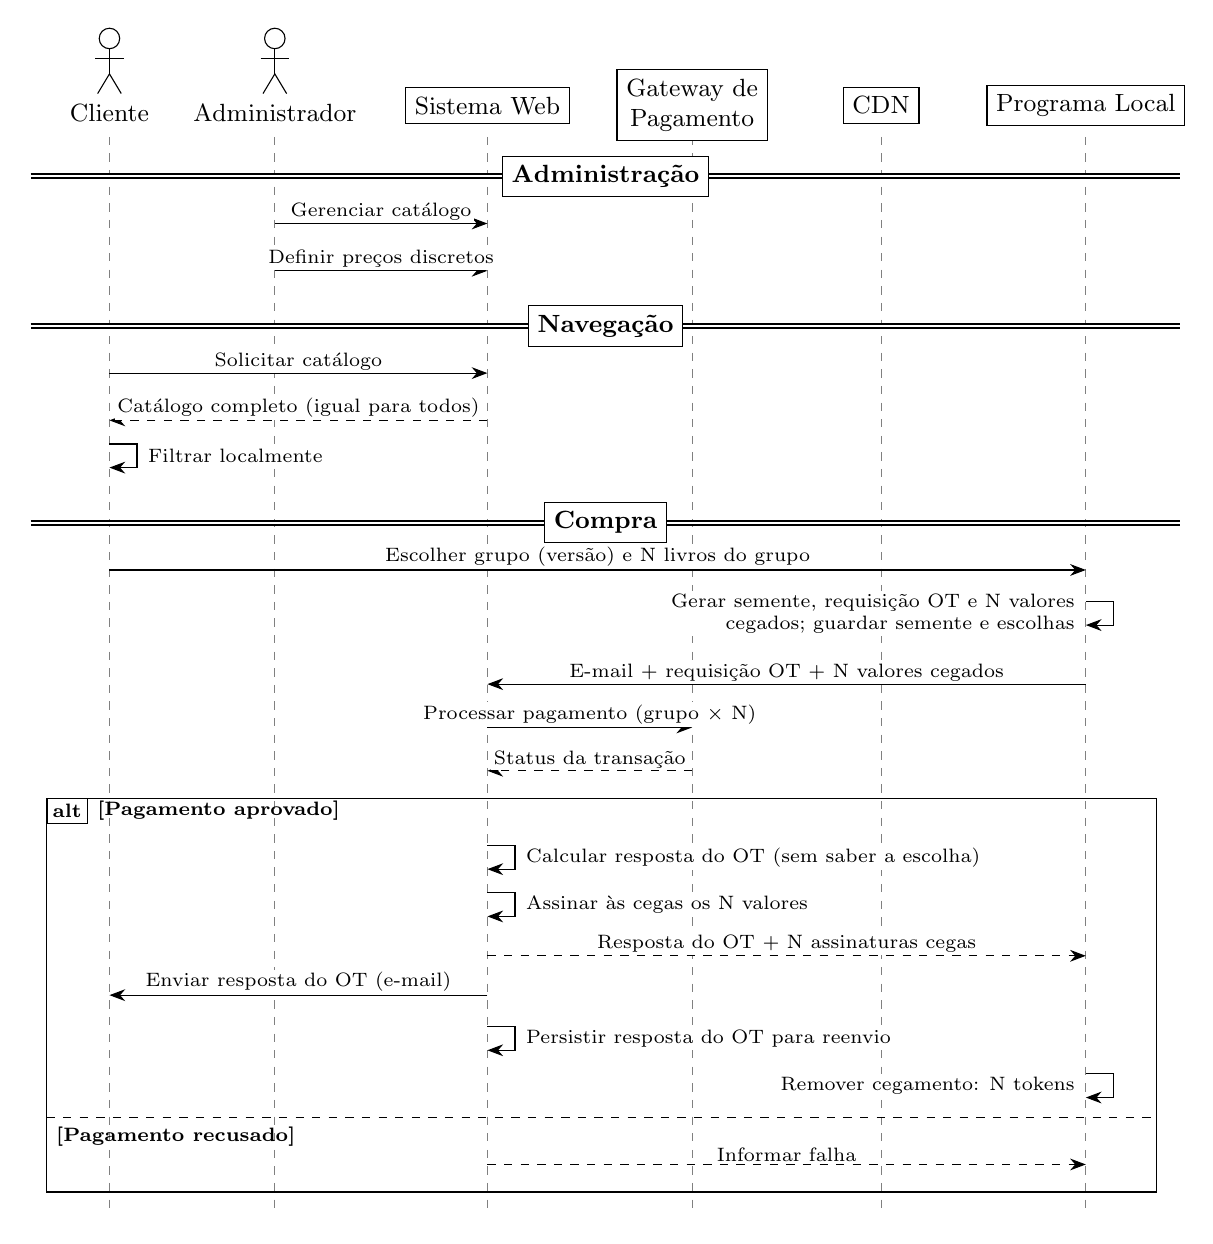
\begin{tikzpicture}
  \sdlifelines{-14.2}
  \sdheads

  \sdbanner{-1.0}{Administração}
  \sdcall{\xAdm}{\xWeb}{-1.6}{Gerenciar catálogo}
  \sdcall{\xAdm}{\xWeb}{-2.2}{Definir preços discretos}

  \sdbanner{-2.9}{Navegação}
  \sdcall{\xCli}{\xWeb}{-3.5}{Solicitar catálogo}
  \sdreply{\xWeb}{\xCli}{-4.1}{Catálogo completo (igual para todos)}
  \sdselfR{\xCli}{-4.4}{Filtrar localmente}

  \sdbanner{-5.4}{Compra}
  \sdcall{\xCli}{\xPrg}{-6.0}{Escolher grupo (versão) e N livros do grupo}
  \sdselfL{\xPrg}{-6.4}{Gerar semente, requisição OT e N valores\\cegados; guardar semente e escolhas}
  \sdcall{\xPrg}{\xWeb}{-7.45}{E-mail + requisição OT + N valores cegados}
  \sdcall{\xWeb}{\xGat}{-8.0}{Processar pagamento (grupo $\times$ N)}
  \sdreply{\xGat}{\xWeb}{-8.55}{Status da transação}

  \sdframe{-0.8}{-8.9}{13.3}{-13.9}{alt}{Pagamento aprovado}
  \sdselfR{\xWeb}{-9.5}{Calcular resposta do OT (sem saber a escolha)}
  \sdselfR{\xWeb}{-10.1}{Assinar às cegas os N valores}
  \sdreply{\xWeb}{\xPrg}{-10.9}{Resposta do OT + N assinaturas cegas}
  \sdcall{\xWeb}{\xCli}{-11.4}{Enviar resposta do OT (e-mail)}
  \sdselfR{\xWeb}{-11.8}{Persistir resposta do OT para reenvio}
  \sdselfL{\xPrg}{-12.4}{Remover cegamento: N tokens}
  \sdelse{-0.8}{13.3}{-12.95}{Pagamento recusado}
  \sdreply{\xWeb}{\xPrg}{-13.55}{Informar falha}
\end{tikzpicture}
\end{figure}

% ---------------------------------------------------------------------------
\begin{figure}[htbp]
\centering
\caption{Diagrama de sequência: entrega, reporte da CDN e descriptografia local}\label{fig:seq-entrega}
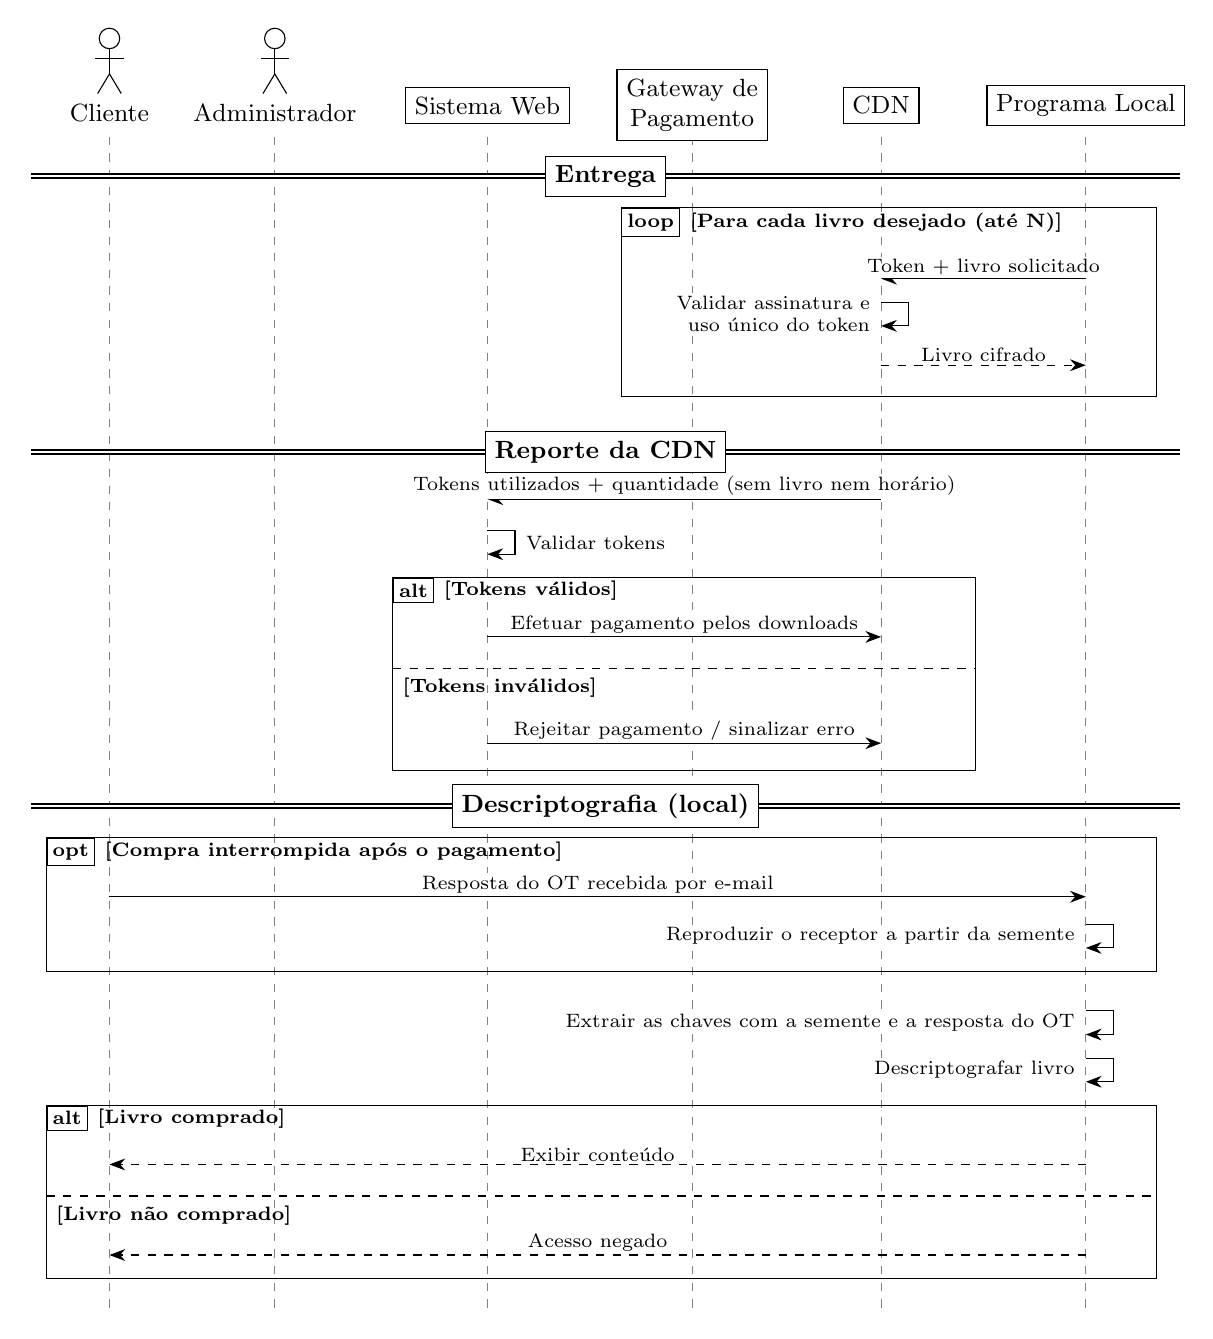
\begin{tikzpicture}
  \sdlifelines{-15.4}
  \sdheads

  \sdbanner{-1.0}{Entrega}
  \sdframe{6.5}{-1.4}{13.3}{-3.8}{loop}{Para cada livro desejado (até N)}
  \sdcall{\xPrg}{\xCdn}{-2.3}{Token + livro solicitado}
  \sdselfL{\xCdn}{-2.6}{Validar assinatura e\\uso único do token}
  \sdreply{\xCdn}{\xPrg}{-3.4}{Livro cifrado}

  \sdbanner{-4.5}{Reporte da CDN}
  \sdcall{\xCdn}{\xWeb}{-5.1}{Tokens utilizados + quantidade (sem livro nem horário)}
  \sdselfR{\xWeb}{-5.5}{Validar tokens}
  \sdframe{3.6}{-6.1}{11.0}{-8.55}{alt}{Tokens válidos}
  \sdcall{\xWeb}{\xCdn}{-6.85}{Efetuar pagamento pelos downloads}
  \sdelse{3.6}{11.0}{-7.25}{Tokens inválidos}
  \sdcall{\xWeb}{\xCdn}{-8.2}{Rejeitar pagamento / sinalizar erro}

  \sdbanner{-9.0}{Descriptografia (local)}
  \sdframe{-0.8}{-9.4}{13.3}{-11.1}{opt}{Compra interrompida após o pagamento}
  \sdcall{\xCli}{\xPrg}{-10.15}{Resposta do OT recebida por e-mail}
  \sdselfL{\xPrg}{-10.5}{Reproduzir o receptor a partir da semente}
  \sdselfL{\xPrg}{-11.6}{Extrair as chaves com a semente e a resposta do OT}
  \sdselfL{\xPrg}{-12.2}{Descriptografar livro}
  \sdframe{-0.8}{-12.8}{13.3}{-15.0}{alt}{Livro comprado}
  \sdreply{\xPrg}{\xCli}{-13.55}{Exibir conteúdo}
  \sdelse{-0.8}{13.3}{-13.95}{Livro não comprado}
  \sdreply{\xPrg}{\xCli}{-14.7}{Acesso negado}
\end{tikzpicture}
\end{figure}

% ===========================================================================
\chapter{Projeto da Solução}\label{cap:projeto}
% ===========================================================================

Este capítulo registra as decisões de projeto tomadas até o momento e as
questões que permanecem em aberto. Ele será expandido com o detalhamento da
implementação e dos resultados das fases 4 e 5.

\section{Decisões de projeto}

\begin{itemize}
\item \textbf{Execução do OT:} síncrona na compra, com o estado do receptor
reproduzível a partir de uma semente guardada pelo programa local (RF11,
RF14).

\item \textbf{Biblioteca de OT:} libOTe \cite{libote}, com o protocolo de
\citeonline{masnyrindal2019} como OT base 1-out-of-2. A compilação no ambiente
do cliente e a reprodutibilidade do receptor a partir da semente são
verificadas por testes automatizados durante a implementação.

\item \textbf{Sistema web:} linguagem Go, banco PostgreSQL, páginas
renderizadas no servidor, sem recursos de terceiros; catálogo entregue por
inteiro e filtrado no cliente; biblioteca de OT acessada por um binário
auxiliar.

\item \textbf{Assinatura cega:} RSA cego padronizado \cite{rfc9474}.

\item \textbf{Programa local:} conecta-se apenas ao sistema web e à CDN.
\end{itemize}

\section{Alternativas descartadas}\label{sec:alternativas}

Esta seção compara, para cada decisão de projeto, a alternativa escolhida com
as descartadas, usando os mesmos critérios para todas. A comparação é
qualitativa: registra propriedades verificadas no código-fonte ou na
documentação de cada alternativa e marca como ``não verificado'' o que não foi
confirmado.

\subsection{Biblioteca de OT}

Critérios:
(C1) compatibilidade com o fluxo de compra, em que o programa local envia a
requisição e o sistema web responde em uma única mensagem;
(C2) possibilidade de guardar ou reproduzir o estado do receptor entre a
requisição e a extração das chaves (RF11, RF14);
(C3) execução no Windows, ambiente do programa local;
(C4) maturidade e recomendação de uso pelos autores;
(C5) aderência ao foco do trabalho, que é o uso de protocolos de OT.

\begin{table}[H]
\centering
\caption{Comparativo das bibliotecas de OT avaliadas}\label{tab:comp-libs}
\footnotesize
\renewcommand{\arraystretch}{1.25}
\begin{tabularx}{\textwidth}{@{}>{\raggedright\arraybackslash}p{0.13\textwidth}
  >{\raggedright\arraybackslash}X >{\raggedright\arraybackslash}X
  >{\raggedright\arraybackslash}p{0.11\textwidth} >{\raggedright\arraybackslash}X
  >{\raggedright\arraybackslash}p{0.11\textwidth}@{}}
\toprule
\textbf{Alternativa} & \textbf{C1 -- Mensagens} & \textbf{C2 -- Estado do receptor} &
\textbf{C3 -- Windows} & \textbf{C4 -- Maturidade} & \textbf{Resultado} \\
\midrule
libOTe, OT base de \citeonline{masnyrindal2019} &
Compatível: a requisição do receptor não depende da mensagem do \emph{sender},
que segue na resposta &
Em memória, mas reproduzível: toda a aleatoriedade do receptor vem do gerador
recebido como parâmetro (verificado no código) &
Sim, segundo os autores &
Acadêmica, licença MIT, amplamente citada &
\textbf{Escolhida} \\
\addlinespace
emp-ot, protocolo PVW &
Compatível: receptor envia primeiro, duas mensagens &
Em memória, chamada bloqueante; reprodutibilidade não verificada &
\textbf{Não} (apenas Linux e macOS) &
Software de pesquisa, sem auditoria independente, segundo os autores &
Descartada (C3) \\
\addlinespace
circl, Simplest OT &
Exige uma troca adicional: a requisição do receptor depende da mensagem inicial
do \emph{sender} &
API dividida em rodadas, favorável &
Sim &
Apenas 1-out-of-2; pacote fora da versão mais recente do módulo &
Descartada (C1, C4) \\
\addlinespace
mpz, Chou--Orlandi &
Mesma dependência da mensagem inicial do \emph{sender} (protocolo Chou--Orlandi) &
Favorável: máquinas de estado sem rede, com mensagens explícitas &
Não verificado &
Autores recomendam não usar em produção; mudanças incompatíveis frequentes &
Descartada (C4) \\
\addlinespace
swanky (Naor--Pinkas, Chou--Orlandi) &
Não verificado &
Não verificado &
Não verificado &
Autores recomendam não usar em produção &
Descartada (C4) \\
\addlinespace
OPRF (RFC 9497) usado para construir 1-out-of-n &
Compatível: cliente envia primeiro, duas mensagens &
API em passos, favorável &
Sim &
Padronizado, várias implementações independentes &
Descartada (C5) \\
\bottomrule
\end{tabularx}
\end{table}

A alternativa baseada em OPRF é tecnicamente adequada, mas não é um protocolo
de OT: ela obtém a funcionalidade de 1-out-of-n a partir de uma função
pseudoaleatória avaliada obliviamente, o que deslocaria o foco do trabalho.

\subsection{Execução do OT}

Critérios: utilidade do envio da resposta por e-mail (RF14) e do reenvio
(RF15); recuperação de uma compra interrompida após o pagamento (RNF07);
quantidade de código criptográfico próprio.

\begin{table}[H]
\centering
\caption{Comparativo das formas de execução do OT}\label{tab:comp-execucao}
\footnotesize
\renewcommand{\arraystretch}{1.25}
\begin{tabularx}{\textwidth}{@{}>{\raggedright\arraybackslash}p{0.2\textwidth}
  >{\raggedright\arraybackslash}X >{\raggedright\arraybackslash}X
  >{\raggedright\arraybackslash}X >{\raggedright\arraybackslash}p{0.12\textwidth}@{}}
\toprule
\textbf{Alternativa} & \textbf{RF14 e RF15} & \textbf{Compra interrompida} &
\textbf{Código criptográfico próprio} & \textbf{Resultado} \\
\midrule
Síncrona, com semente guardada &
Úteis: a resposta recebida por e-mail permite extrair as chaves &
Recuperável a partir da semente &
Nenhum além de inicializar o gerador com a semente; depende da premissa de
determinismo do receptor &
\textbf{Escolhida} \\
\addlinespace
Síncrona, sem estado guardado &
Perdem a utilidade: sem o segredo, a resposta não serve &
Irrecuperável: o cliente paga e perde a compra &
Nenhum &
Descartada \\
\addlinespace
Adaptador com estado serializado &
Úteis &
Recuperável a partir do estado salvo &
Reorganização do protocolo em duas etapas sobre as primitivas da biblioteca &
Descartada \\
\bottomrule
\end{tabularx}
\end{table}

\subsection{Onde executa o receptor do OT}

Critérios: natureza da privacidade da escolha (RF07), usabilidade, viabilidade
técnica com a biblioteca escolhida e armazenamento da semente (RF11).

\begin{table}[H]
\centering
\caption{Comparativo dos locais de execução do receptor}\label{tab:comp-receptor}
\footnotesize
\renewcommand{\arraystretch}{1.25}
\begin{tabularx}{\textwidth}{@{}>{\raggedright\arraybackslash}p{0.19\textwidth}
  >{\raggedright\arraybackslash}X >{\raggedright\arraybackslash}X
  >{\raggedright\arraybackslash}X >{\raggedright\arraybackslash}X
  >{\raggedright\arraybackslash}p{0.11\textwidth}@{}}
\toprule
\textbf{Alternativa} & \textbf{Privacidade da escolha} & \textbf{Usabilidade} &
\textbf{Biblioteca de OT} & \textbf{Semente} & \textbf{Resultado} \\
\midrule
Programa local com acesso restrito ao sistema web e à CDN &
Garantia do protocolo &
Sem transporte manual de arquivos &
Execução nativa &
Disco do cliente &
\textbf{Escolhida} \\
\addlinespace
Programa local sem rede (versão 2 desta especificação) &
Garantia do protocolo &
Cliente transporta arquivos entre navegador e programa &
Execução nativa &
Disco do cliente &
Descartada \\
\addlinespace
Navegador, com código fornecido pelo sistema web &
Premissa: o servidor fornece código honesto &
Nada a instalar &
Exigiria compilação para WebAssembly (viabilidade não verificada) &
Guardada no navegador, sujeita a remoção &
Descartada \\
\addlinespace
Navegador, com código de outra origem (extensão ou página estática auditável) &
Premissa mais fraca: código auditável e independente do servidor &
Instalação de extensão ou uso de página separada &
Mesma limitação da alternativa anterior &
Guardada no navegador &
Descartada \\
\bottomrule
\end{tabularx}
\end{table}

\subsection{Tecnologias do sistema web}

\begin{table}[H]
\centering
\caption{Comparativo das tecnologias do sistema web}\label{tab:comp-stack}
\footnotesize
\renewcommand{\arraystretch}{1.25}
\begin{tabularx}{\textwidth}{@{}>{\raggedright\arraybackslash}p{0.14\textwidth}
  >{\raggedright\arraybackslash}p{0.2\textwidth} >{\raggedright\arraybackslash}p{0.2\textwidth}
  >{\raggedright\arraybackslash}X@{}}
\toprule
\textbf{Tema} & \textbf{Escolhida} & \textbf{Descartada} & \textbf{Motivo} \\
\midrule
Linguagem & Go & TypeScript (Node.js); Python &
Go oferece assinatura cega RSA padronizada \cite{rfc9474} em biblioteca
mantida, biblioteca padrão com servidor HTTP e criptografia, e binário único.
Em Python não foi identificada implementação consolidada da RFC 9474. \\
\addlinespace
Banco de dados & PostgreSQL & SQLite &
Escritas concorrentes representativas para o teste de carga (RNF05). \\
\addlinespace
Interface & HTML gerado no servidor & Aplicação de página única (SPA) &
Menor superfície de ataque e nenhuma dependência de código de terceiros no
navegador. \\
\addlinespace
Busca (RF04) & Catálogo inteiro, filtrado no cliente & Busca no servidor sem
registros &
Na busca no servidor, o sistema web observa as consultas; a proteção
dependeria apenas de disciplina operacional. \\
\addlinespace
Acesso à biblioteca de OT & Binário auxiliar & Ligação direta ao código C++ &
Isola o código C++ e desacopla a compilação da biblioteca da compilação do
sistema web. \\
\bottomrule
\end{tabularx}
\end{table}

\section{Questões em aberto}

\begin{itemize}
\item Variante de OT: 1-out-of-n repetido (por exemplo, a construção de
\citeonline{naorpinkas1999} sobre 1-out-of-2), k-out-of-n ou GOT.
\item Algoritmo simétrico para cifrar os livros, dentro de RNF01.
\item Formato dos artefatos: requisição OT, resposta OT, tokens e livro
cifrado.
\item Tamanho mínimo de um grupo de mesmo preço.
\item Política de chaves da assinatura cega e tamanho do conjunto de
anonimato dos tokens.
\item Token de uso único ou com novo download do mesmo livro.
\item Frequência e lotes do reporte da CDN e remuneração por token.
\item Prazo de reenvio da resposta do OT (RF15).
\item Gateway de pagamento e sua integração com o programa local.
\item Proteção da semente armazenada no programa local.
\end{itemize}

% ---------------------------------------------------------------------------
\postextual
\bibliography{referencias}

\end{document}
